\documentclass[11pt]{article}
\usepackage[margin=1in]{geometry}
\usepackage{graphicx}
\usepackage{booktabs}
\usepackage{hyperref}
\usepackage{parskip}

\title{\textbf{CS 8803 HML - Lab 3}}
\author{}
\date{}

\begin{document}
\maketitle

%% ─────────────────────────────────────────────
\section*{Screenshots}

\begin{figure}[h]
    \centering
    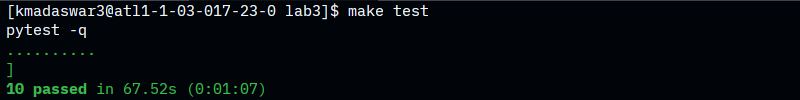
\includegraphics[width=0.85\linewidth]{screenshots/test.png}
    \caption{Pytest Results}
\end{figure}

\begin{figure}[h]
    \centering
    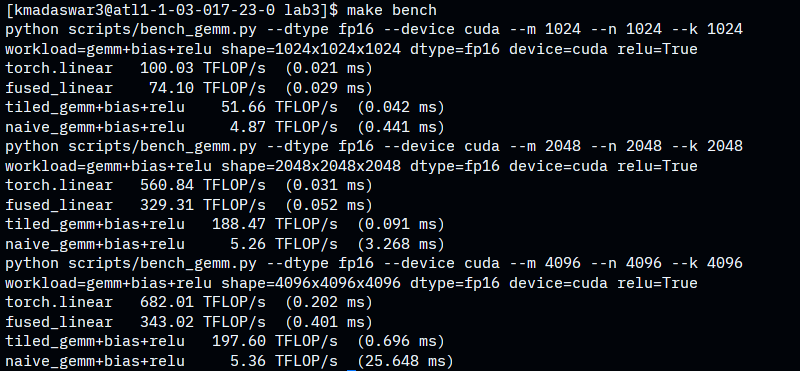
\includegraphics[width=0.85\linewidth]{screenshots/bench.png}
    \caption{Benchmark Results}
\end{figure}

\begin{figure}[h]
    \centering
    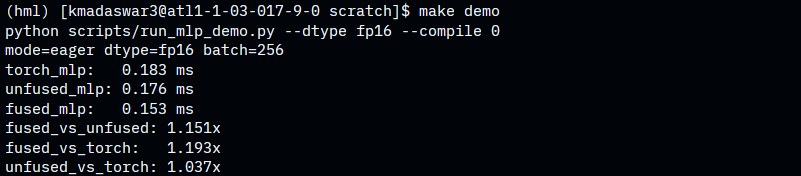
\includegraphics[width=0.85\linewidth]{screenshots/demo.png}
    \caption{MLP Demo Results}
\end{figure}

%% ─────────────────────────────────────────────
\section*{Kernel Design}

\subsection*{1. Naive GEMM (\texttt{gemm\_naive.py})}

The naive kernel computes each output element by iterating over the shared K dimension
one scalar at a time, multiplying the corresponding elements of A and B and accumulating
the result. It never uses tensor cores, so performance is bottlenecked by scalar arithmetic
and tops out around 5 TFLOP/s regardless of matrix size.

\subsection*{2. Tiled GEMM (\texttt{gemm\_tiled.py})}

Instead of working scalar by scalar, the tiled kernel loads rectangular blocks of A and B
into registers and uses \texttt{tl.dot()} to multiply them. Unlike the naive per-element
multiply-accumulate, \texttt{tl.dot()} issues a single warp-level matrix multiply
instruction that dispatches to the GPU's tensor cores, which can compute thousands of FMAs
in one instruction. This single change improves throughput by 40$\times$ over the naive kernel.

\subsection*{3. Fused GEMM (\texttt{gemm\_fused.py})}

Builds on the tiled kernel by adding the bias addition and ReLU activation into the same
kernel rather than launching them as separate operations. Since the result of the matrix
multiply is already in registers, applying bias and ReLU there avoids writing intermediate
results to global memory just to read them back. This gives a speedup
of 1.16$\times$ over the unfused path and 1.12$\times$ over PyTorch's \texttt{nn.Linear}.

%% ─────────────────────────────────────────────
\section*{Profiling Analysis}

Profiled on a $4096 \times 4096 \times 4096$ fp16 GEMM (NVIDIA H200).

\begin{table}[h]
\centering
\begin{tabular}{lcc}
\toprule
\textbf{Metric} & \textbf{Naive} & \textbf{Tiled} \\
\midrule
Duration              & 33.70 ms   & 0.78 ms     \\
Compute Throughput    & 89.63\%    & 24.56\%     \\
Memory Throughput     & 80.52\%    & 91.84\%     \\
Memory BW (effective) & 23.11 GB/s & 253.98 GB/s \\
Achieved Occupancy    & 98.72\%    & 48.47\%     \\
\bottomrule
\end{tabular}
\caption{Nsight Compute metrics for naive and tiled GEMM kernels.}
\end{table}

\textbf{Naive kernel:} High compute throughput (89.6\%) and occupancy (98.7\%) are
misleading as the kernel is busy doing scalar FMAs rather than tensor core MACs. Despite
high utilization, effective memory bandwidth is only 23 GB/s because loads are serialized
one element at a time across K. The result is a 33.7 ms runtime for a problem that the
tiled kernel solves in under 1 ms.

\textbf{Tiled kernel:} Memory throughput jumps to 91.8\% with 254 GB/s effective
bandwidth, while compute throughput drops to 24.6\%, showing the kernel is now
memory-bound. \texttt{tl.dot()} dispatches to tensor cores which are fast enough to
consume each tile before the next one arrives from memory, leaving the SM stalled waiting
on loads rather than doing compute. Occupancy falls to 48.5\% because holding the large
accumulator tile in registers across the K loop requires 64 registers per thread (vs.\ 32
for naive), which halves the number of warps that can fit on the SM simultaneously.

%% ─────────────────────────────────────────────
\section*{Optimization Attempts and Improvement Ideas}

\begin{enumerate}

\item \textbf{Software pipelining (\texttt{num\_stages}):} Increasing \texttt{num\_stages}
in the tiled kernel lets Triton overlap global-memory loads for the next tile with the
\texttt{tl.dot()} compute for the current tile. Increasing \texttt{num\_stages} from 1 to
2 improved throughput from 218 to 331 TFLOP/s, but returns diminish beyond that because
each additional stage consumes more shared memory, reducing the number of concurrent blocks
per SM and lowering occupancy.

\item \textbf{Block size tuning:} Increasing \texttt{BLOCK\_M=BLOCK\_N} from 64 to 128
and \texttt{BLOCK\_K} from 32 to 64 improves tensor-core utilization by performing more
useful work per block, speeding up the kernel from 342 to 454 TFLOP/s on shape
$4096\times4096\times4096$. The benefit is not visible for smaller shapes like
$1024\times1024\times1024$ because larger tiles produce fewer total blocks
($8\times8=64$ vs $16\times16=256$), leaving most of the 132 SMs idle.

\end{enumerate}

\end{document}
